%%%%%%%%%%%%%%%%%%%%%%%%%%%%%%%%%%%%%%%%%
% Beamer Presentation
% LaTeX Template
% Version 1.0 (10/11/12)
%
% This template has been downloaded from:
% http://www.LaTeXTemplates.com
%
% License:
% CC BY-NC-SA 3.0 (http://creativecommons.org/licenses/by-nc-sa/3.0/)
%
%%%%%%%%%%%%%%%%%%%%%%%%%%%%%%%%%%%%%%%%%

%----------------------------------------------------------------------------------------
%	PACKAGES AND THEMES
%----------------------------------------------------------------------------------------


% The Beamer class comes with a number of default slide themes
% which change the colors and layouts of slides. Below this is a list
% of all the themes, uncomment each in turn to see what they look like.

%\usetheme{default}
%\usetheme{AnnArbor}
%\usetheme{Antibes}
%\usetheme{Bergen}
%\usetheme{Berkeley}
%\usetheme{Berlin}
%\usetheme{Boadilla}
%\usetheme{CambridgeUS}
%\usetheme{Copenhagen}
%\usetheme{Darmstadt}
%\usetheme{Dresden}
%\usetheme{Frankfurt}
%\usetheme{Goettingen}
%\usetheme{Hannover}
%\usetheme{Ilmenau}
%\usetheme{JuanLesPins}
%\usetheme{Luebeck}
%\usetheme{Madrid}
%\usetheme{Malmoe}
%\usetheme{Marburg}
%\usetheme{Montpellier}
%\usetheme{PaloAlto}
%\usetheme{Pittsburgh}
%\usetheme{Rochester}
%\usetheme{Singapore}
%\usetheme{Szeged}
%\usetheme{Warsaw}

% As well as themes, the Beamer class has a number of color themes
% for any slide theme. Uncomment each of these in turn to see how it
% changes the colors of your current slide theme.

%\usecolortheme{albatross}
%\usecolortheme{beaver}
%\usecolortheme{beetle}
%\usecolortheme{crane}
%\usecolortheme{dolphin}
%\usecolortheme{dove}
%\usecolortheme{fly}
%\usecolortheme{lily}
%\usecolortheme{orchid}
%\usecolortheme{rose}
%\usecolortheme{seagull}
%\usecolortheme{seahorse}
%\usecolortheme{whale}
%\usecolortheme{wolverine}

%\setbeamertemplate{footline} % To remove the footer line in all slides uncomment this line
%\setbeamertemplate{footline}[page number] % To replace the footer line in all slides with a simple slide count uncomment this line

%\setbeamertemplate{navigation symbols}{} % To remove the navigation symbols from the bottom of all slides uncomment this line


%%----------------------------------------------------------------------------------------
%	TITLE PAGE
%----------------------------------------------------------------------------------------
\begin{frame}
\title[Introduction to \LaTeX]{Introduction to \LaTeX} % The short title appears at the bottom of every slide, the full title is only on the title page
\subtitle{Winter School Modelling Hub 2021}
%\author{Winter School Modelling Hub 2021} % Your name
\institute[Antarctica Research Centre]{Victoria University of Wellington} % Your institution as it will appear on the bottom of every slide, may be shorthand to save space
%{Victoria University of Wellington} \\ % Your institution for the title page
%\medskip
%\textit{angela.bahamondesdominguez@niwa.co.nz} % Your email address
\titlegraphic{
    
\includegraphics[width=6cm]{figures/overleaf_logo.png}
}
%\logo{
%
\includegraphics[width=6cm]{figures/overleaf_logo.png}}
\date{} % Date, can be changed to a custom date
\end{frame}

\begin{frame}
\titlepage % Print the title page as the first slide
\end{frame}

%\begin{frame}
%\frametitle{Why \LaTeX?} % Table of contents slide, comment this block out to remove it
%\tableofcontents % Throughout your presentation, if you choose to use \section{} and \subsection{} commands, these will automatically be printed on this slide as an overview of your presentation
%\end{frame}

%----------------------------------------------------------------------------------------
%	PRESENTATION SLIDES
%----------------------------------------------------------------------------------------

%------------------------------------------------
%\section{First Section} % Sections can be created in order to organize your presentation into discrete blocks, all sections and subsections are automatically printed in the table of contents as an overview of the talk
%------------------------------------------------

%\subsection{Subsection Example} % A subsection can be created just before a set of slides with a common theme to further break down your presentation into chunks

\begin{frame}[fragile]
\frametitle{What is \LaTeX?}
\begin{itemize}
\item Is a typesetting language. \\
\item When using \LaTeX, you write a plain text file which describes the document's structure and presentation. \LaTeX{} converts this source text into a typeset document. \\
\end{itemize}

For example: \\
\color{purple}
The IPCC assess the science related to \verb!\textit{climate change}!.\\ 
\color{black}
\begin{center}
	$\big\Downarrow$
\end{center}
\color{purple}
\begin{center}
The IPCC assess the science related to \textit{climate change}. \\
\end{center} 
 \end{frame} 

%------------------------------------------------

\begin{frame}[fragile]
\frametitle{Why \LaTeX?}
\begin{itemize}
\item \LaTeX{} is created by scientists, for scientists and there is a large and active community. \\
\pause
\item Is open source, you can find all commonly and most rarely used features online. \\
\pause
\item It makes it very simple to handle equations, figures, references, etc. References are handled by BibDesk (Mac users) and it can read EndNote. \\
\pause
\item The consistency of the layout: you focus on the content of the document and let \LaTeX{} focus how to handle how the output is formatted.\\
\pause
\item It is a powerful program, you can extend it to write papers, articles, presentations, etc.\\
\pause
\item To write huge documents (master, PhD thesis) you can have a file per chapter and join them together with just one click!\\
\pause
\item In some journals, you might pay less to publish if your manuscript is done in \LaTeX{} instead of Word (e.g. half the price per page in \LaTeX{} than it is in Word).
\end{itemize}
\end{frame}

%------------------------------------------------

\begin{frame}[fragile]
\frametitle{How does it work?}
\begin{verbnobox}[\vbdelim]
<\documentclass{>article<} % style of the document>
<\begin{>document<} %command to start the doc>
Hello World <% your content goes here>
<\end{>document<}>
\end{verbnobox}
\pause
\textbf{Some tips:} 
\begin{itemize}
\item Commands start with  \color{blue}{\verb|\|} \\ 
\color{black}
\item Every doc starts with \color{blue}{\verb|\documentclass|} \\
\color{black}
\item The sign \color{blue}{\verb|%|} \color{black} starts a comment \\
\item Special characters: \color{blue}{\verb|%, $, &, #, _, {, }, \|}. \color{black} Need to be written as: \color{blue}{\verb|\%, \$, \&, \#, \_, \{, \}, \textbackslash|}
\end{itemize}
\end{frame}

%------------------------------------------------
\begin{frame}[fragile]
\frametitle{Preamble of the document}
\begin{itemize}
\item The part of your .tex before the \verb|\begin{document}| command is called the \textbf{preamble}.
\end{itemize}
The following command: 
\begin{framed}
\begin{minipage}[b]{.4\textwidth}
\begin{verbnobox}[\vbdelim]
<\documentclass>[12pt, letterpaper]<{>article<}> 
\end{verbnobox}
\end{minipage}% This must go next to `\end{minipage}`
\end{framed}

\begin{itemize}
\item Defines the type of document.\\
\item Inside the squared brackets you can define the font size (12pt). The default is 10pt. \\
\item You can also define the paper size (letterpaper). Other values can be A4 and legalpaper. Default is A4. \\
\item If you want to use the default parameters, you can ignore the squared brackets.
\end{itemize}
\end{frame}

%------------------------------------------------
\begin{frame}[fragile]
\frametitle{Preamble of the document}
Document types available in the \color{blue}{\verb|\documentclass|} \color{black}{command:} \\
\vspace{1cm}
\begin{tabular}{ll}
\textbf{Document type} & \textbf{Description} \\ \hline
article & For short documents and journal articles \\ 
report & For longer documents and dissertations \\ 
book & Useful to write books \\
letter & For letters \\ 
slides & For slides, rarely used \\ 
beamer & Slides in the Beamer class format \\ \hline
\end{tabular}

The document type 'article' is the most commonly used!
\end{frame}


%------------------------------------------------

\begin{frame}[fragile]
\frametitle{More examples of commands and their outputs}
%\begin{center}
\begin{framed}
\begin{minipage}[b]{.4\textwidth}
%\raggedright
  \begin{verbnobox}[\vbdelim]
<\begin{>itemize<}>
<\item> Clouds 
<\item> Ocean 
<\item> Volcanoes 
<\end{>itemize<}>  
\end{verbnobox}
\end{minipage}% This must go next to `\end{minipage}`
\end{framed}
\begin{framed}
\begin{minipage}[b]{.4\textwidth}
   % \raggedleft
%\begin{center}
%	$\big\Downarrow$
%\end{center}
\begin{itemize}
\item Clouds \\
\item Ocean \\
\item Volcanoes \\
\end{itemize}
\end{minipage}
\end{framed}
%\end{center}
\end{frame}

%------------------------------------------------

\begin{frame}[fragile]
\frametitle{More examples of commands and their outputs}
\begin{framed}
\begin{minipage}[b]{.4\textwidth}
  \begin{verbnobox}[\vbdelim]
<\begin{>equation<}>
<\alpha> + <\beta> + 1  
<\end{>equation<}>  
\end{verbnobox}
\end{minipage}% This must go next to `\end{minipage}`
\end{framed}
\begin{framed}
\begin{minipage}[b]{.4\textwidth}
\begin{equation}
\alpha + \beta + 1
\end{equation}
\end{minipage}
\end{framed}
\end{frame}


%------------------------------------------------
\begin{frame}[fragile]
\frametitle{More examples of commands and their outputs}
\begin{framed}
\begin{minipage}[b]{.4\textwidth}
  \begin{verbnobox}[\vbdelim]
<\begin{>figure<}>
<\includegraphics>[width=50mm]<{>figures/cat.jpeg<}>
<\end{>figure<}>
\end{verbnobox}
\end{minipage}% This must go next to `\end{minipage}`
\end{framed}
\begin{framed}
\begin{minipage}[b]{.1\textwidth}
\begin{figure}

\includegraphics[width=50mm]{figures/cat.jpeg}
\end{figure}
\end{minipage}
\end{framed}
\end{frame}

%------------------------------------------------

\begin{frame}[fragile] % Need to use the fragile option when verbatim is used in the slide
\frametitle{What about errors? }
\begin{enumerate}
\item \LaTeX{} will stop compiling if there is an error. 
\item For example, if you misspell a command or forget a bracket, \LaTeX{} will stop with a message error showing the line and explaining the error (most of the times!).
\item Advice? Fix errors as soon as they arise.
\end{enumerate}
\end{frame}

%------------------------------------------------

\begin{frame}
\frametitle{Exercise 1: Overleaf}
\begin{itemize}
\item Open the exercise in Overleaf (Exercise1.tex).
\item Compile and fix the errors.
\item  Hint: Watch out for characters with special meanings ...
\end{itemize}

\textbf{Exercise 1}
\noindent\fbox{%
    \parbox{\textwidth}{%
        Female academics earn \$400,000 less than men over life-time. And of professors, only 28\% were female in 2019/20.    }}
\end{frame}

%------------------------------------------------

\begin{frame}[fragile] % Need to use the fragile option when verbatim is used in the slide
\frametitle{Packages}
\begin{itemize}
\item \textit{Packages} are libraries of extra commands and environments. \\
\item We need to load the packages in the \textit{preamble} as: \color{blue}{\verb|\usepackage{}|} \color{black}{}. The name of the package goes inside the curly brackets. \\
\item There are two categories of \textit{packages}: 
\begin{enumerate}
\item Packages that allow you to change the layout or structure of your document. For example, \color{red}{multicol} \color{black}{}. \\
\item Packages that allow you include new or enhanced content within your document. For example, \color{red}{amsmath} \color{black}{}.  \\
\end{enumerate}
\color{black}
\end{itemize}
\end{frame}

%------------------------------------------------
\begin{frame}[fragile] % Need to use the fragile option when verbatim is used in the slide
\frametitle{Packages}
\begin{itemize}
\item Example for \color{red}{multicol} \color{black}{}: \\
\end{itemize}
\begin{verbnobox}[\vbdelim]
<\documentclass{>article<}>
<\usepackage{>multicol<}> % preamble
<\begin{>document<}>
<\begin{>multicols<}{>2<}>
% Anything you write here will be in two columns
<\end{>multicols<}>   
<\end{>document<}>
\end{verbnobox}  %
\pause
\begin{itemize}
\item Example: \color{red}{\verb|amsmath|} \color{black}{} for maths! \\
\end{itemize}

\begin{verbnobox}[\vbdelim]
<\documentclass{>article<}>
<\usepackage{>amsmath<}> % preamble
<\begin{>document<}>
% write your equations here!
<\end{>document<}>
\end{verbnobox}  %

\end{frame}

%------------------------------------------------
\begin{frame}[fragile]
\frametitle{More packages}
\begin{itemize}
\item \verb|beamer| for presentations  \\
\item \verb|tikz| for amazing graphics \\
\item \verb|spreadtab| to create spreadsheets \\
\item \verb|listings| as a source code printer for \LaTeX \\
\item \verb|cwpuzzle| for crossword puzzles (not that I have used it before!) \\
\end{itemize}
\end{frame}
%------------------------------------------------

\begin{frame}[fragile]
\frametitle{Enviroments}
\begin{itemize}
\item The dollar sign (\color{red}{\$}\color{black}{}) is special, because we can use it to mark math in the text.\\
\item If you want to write a small equation in the text, always use dollar signs in pairs:
\end{itemize}
\begin{framed}
\begin{minipage}[b]{.4\textwidth}
\begin{verbnobox}[\vbdelim]
Let <$>y=mx+b<$> be <\ldots>
\end{verbnobox}
\end{minipage}% This must go next to `\end{minipage}`
\end{framed}
\begin{framed}
\begin{minipage}[b]{.4\textwidth}
Let $y=mx+b$ be \ldots
\end{minipage}
\end{framed}
\begin{itemize}
\item However, if your equation is big and scary, use the \verb|equation| enviroment as: 
\end{itemize}

\begin{verbnobox}[\vbdelim]
<\begin{>equation<}>
% equation goes here
<\end{>equation<}>
\end{verbnobox}
\end{frame}

%------------------------------------------------
\begin{frame}[fragile]
\frametitle{Exercise 2: Overleaf}
\begin{itemize}
\item Open the exercise in Overleaf (Exercise2.tex).
\item Write the following equation.
\item  Hint: A fraction is written as \verb|\frac{num}{den}| and a partial derivative is \verb|\partial|.
\end{itemize}

\textbf{Exercise 2}
\noindent\fbox{%
    \parbox{\textwidth}{%
        The momentum equation for vertical velocity is:  
        \begin{equation}
        \frac{\partial w}{\partial t} + u\frac{\partial w }{\partial x} + v\frac{\partial w}{\partial y} + w\frac{\partial w}{\partial z}=-\frac{1}{\rho}\frac{\partial p}{\partial z}+2\Omega u \cos(\gamma) -g
        \end{equation}
        }}
\end{frame}

%------------------------------------------------
\begin{frame}[fragile]
\frametitle{Exercise 2: Overleaf}
\begin{figure}
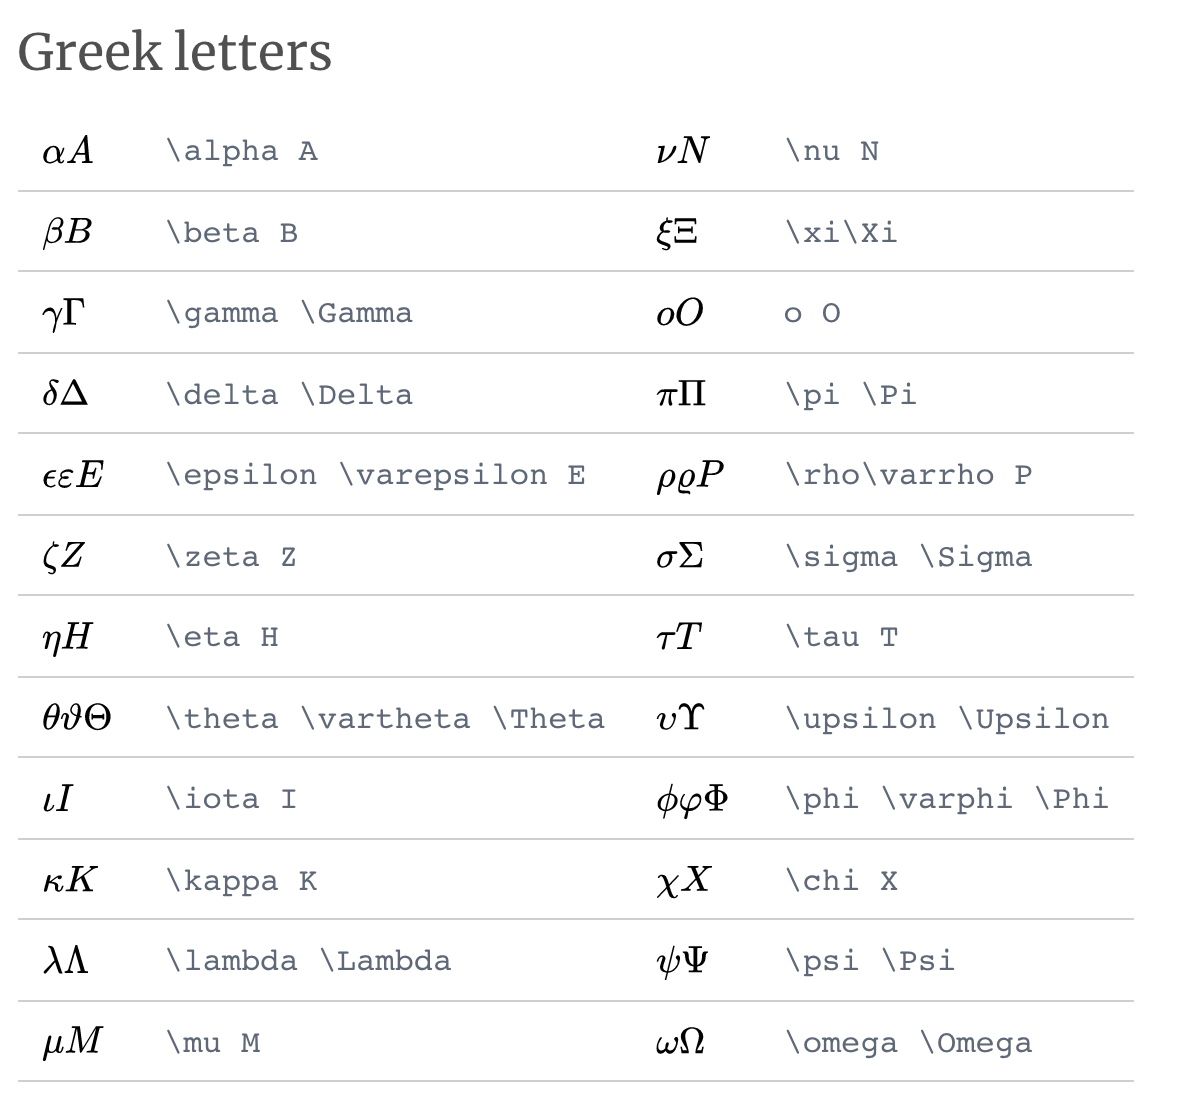
\includegraphics[width=90mm]{figures/Greek.png}
\end{figure}
\end{frame}
%------------------------------------------------
\begin{frame}[fragile]
\frametitle{Graphics}
\begin{itemize}
\item Use the  \verb|graphicx| package, which provides the \color{blue}{\verb|\includegraphics[keys=value, ...]{file-name}|} \color{black} command. \\
\item The \verb|graphicx| package supports different formats: JPEG, PNG, PDF. \\
\item Note that the optional parameter accepts a comma separated list of \textit{keys} and associated \textit{values}.\\
\item Some of the most important \textit{keys} include: \verb|width|, \verb|height|, \verb|angle|, \verb|scale|. \\
\end{itemize}
\begin{framed}
\begin{verbnobox}[\vbdelim]
<\begin{>figure<}>
<\includegraphics>[width=0.5<\textwidth>]<{>image.png<}>
<\caption{>Caption of the figure goes here.<}>
<\end{>figure<}>
\end{verbnobox}
\end{framed}
The command $width=0.5$ makes the image take up 50\% of the width of the surrounding text ( \color{blue}{\verb|\textwidth|}\color{black}).
\end{frame}

%------------------------------------------------
\begin{frame}[fragile]
\frametitle{Tables}
\begin{itemize}
\item Tables can be tricky, but do not worry as everything comes with some practice. \\
\item  You need to add the package: \color{red}{\verb|tabularx|} \color{black}{}
\end{itemize}

\begin{framed}
\begin{minipage}[b]{.4\textwidth}
\begin{verbnobox}[\vbdelim]
<\begin{>tabular<}{>lrr<}>
Item <&> Qty <&> Unit <\$ \\>
Widget <&> 1 <&> 199.99 <\\>
Gadget <&> 2 <&> 399.99 <\\>
Cable <&> 3 <&> 19.99 <\\>
<\end{>tabular<}>
\end{verbnobox}
\end{minipage}% This must go next to `\end{minipage}`
\end{framed}
\pause
\begin{framed}
\begin{minipage}[b]{.4\textwidth}
\begin{tabular}{lrr}
Item & Qty & Unit \$ \\
Widget & 1 & 199.99 \\
Gadget & 2 & 399.99 \\
Cable & 3 & 19.99 \\
\end{tabular}
\end{minipage}
\end{framed}
\end{frame}



%------------------------------------------------
\begin{frame}[fragile]
\frametitle{Tables}
\begin{itemize}
\item You can add horizontal lines with \color{blue}{\verb|\hline|} \color{black}
\end{itemize}
\begin{framed}
\begin{minipage}[b]{.4\textwidth}
\begin{verbnobox}[\vbdelim]
<\begin{>tabular<}{>| l | r | r |<}> <\hline>
Item <&> Qty <&> Unit <\$ \\ \hline>
Widget <&> 1 <&> 199.99 <\\ \hline>
Gadget <&> 2 <&> 399.99 <\\ \hline>
Cable <&> 3 <&> 19.99 <\\ \hline>
<\end{>tabular<}>
\end{verbnobox}
\end{minipage}% This must go next to `\end{minipage}`
\end{framed}
\pause
\begin{framed}
\begin{minipage}[b]{.4\textwidth}
\begin{tabular}{| l | r | r |} \hline
Item & Qty & Unit \$ \\ \hline
Widget & 1 & 199.99 \\ \hline
Gadget & 2 & 399.99 \\ \hline
Cable & 3 & 19.99 \\ \hline
\end{tabular}
\end{minipage}
\end{framed}
\end{frame}


%------------------------------------------------
\begin{frame}[fragile]
\frametitle{Structured documents}
\begin{itemize}
\item \color{blue}{\verb|\title|} \color{black}and \color{blue}{\verb|\author|} \color{black} go in the \textit{preamble}.\\
\item We can use \color{blue}{\verb|\maketitle|} \color{black} to create the title. \\
\end{itemize}
\begin{framed}
\begin{minipage}[b]{0.4\textwidth}
\begin{verbnobox}[\vbdelim]
<\documentclass{>article<}>
<\title{>The title<}>
<\author{>Author<}>
<\date{\today}>
<\begin{>document<}>
<\maketitle>
<\begin{>abstract<}>
Abstract goes here!
<\end{>abstract<}>
\end{verbnobox}
\end{minipage}% This must go next to `\end{minipage}`
\end{framed}
\end{frame}

%------------------------------------------------
\begin{frame}[fragile]
\frametitle{Structured documents}
\begin{figure}
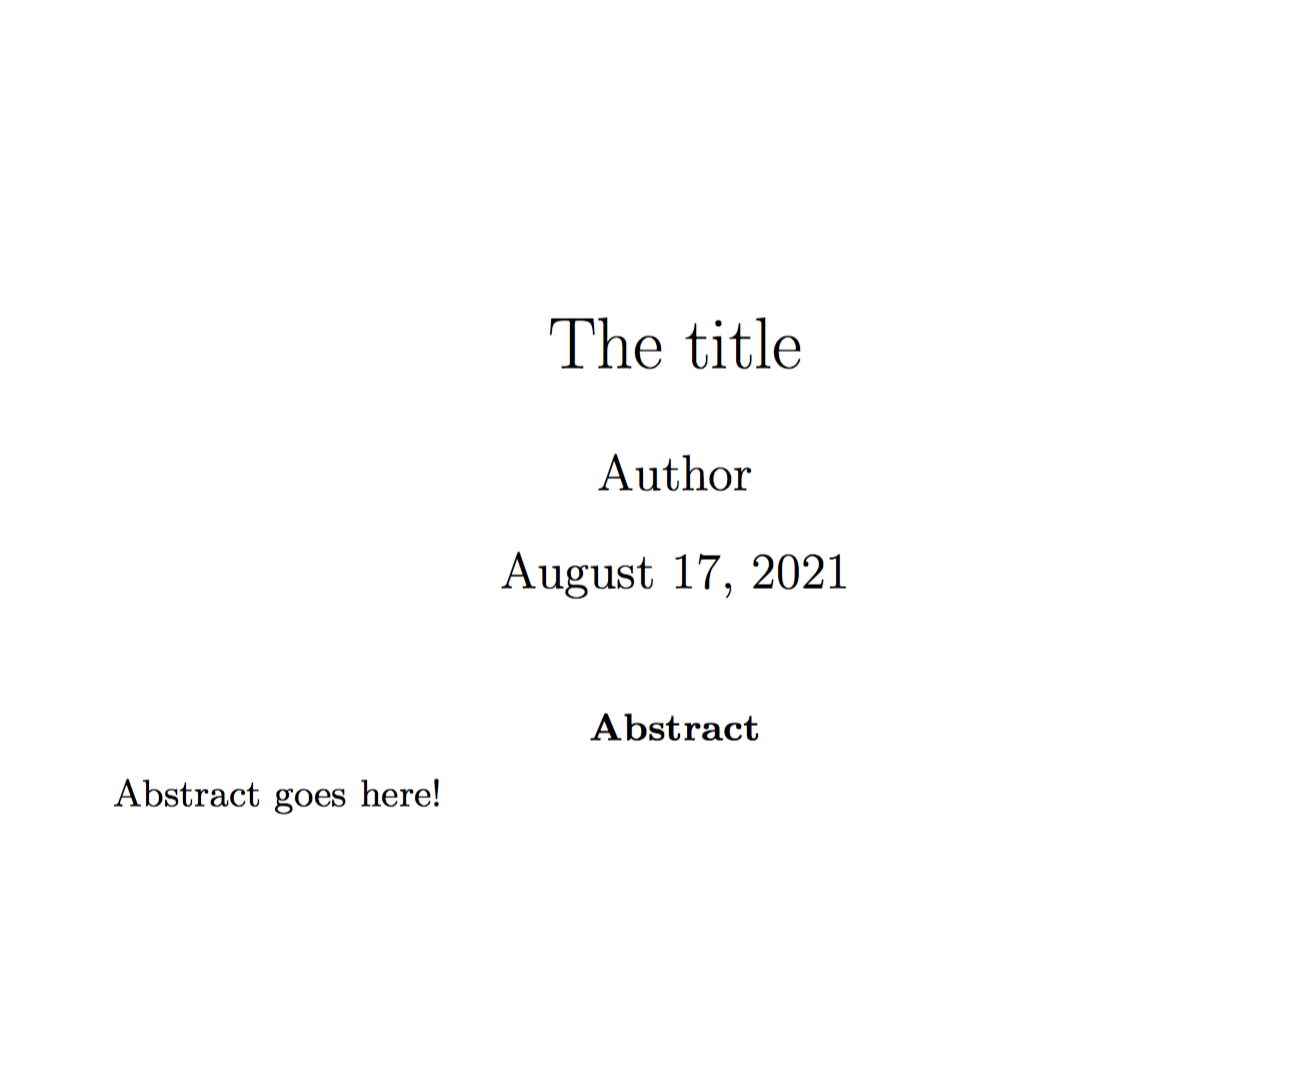
\includegraphics[width=100mm]{figures/example.png}
\end{figure}
\end{frame}


%------------------------------------------------
\begin{frame}[fragile]
\frametitle{Sections}
\begin{itemize}
\item You can use the \color{blue}{\verb|\section|} \color{black}and \color{blue}{\verb|\subsection|} \color{black} commands (or \color{blue}{\verb|\subsubsection|}\color{black}? depending on how brave you are!).\\
\item When you write \color{blue}{\verb|\section*|} \color{black}or \color{blue}{\verb|\subsection*|} \color{black}it means that it will not be numerated. \\
\end{itemize}

\begin{framed}
\begin{verbnobox}[\vbdelim]
<\documentclass{>article<}>
<\begin{>document<}>
<\section{>Introduction<}>
I always struggle with intros <\ldots>
<\section{>Methods<}>
Whatever methods you used <\ldots>
<\subsection{>Fieldwork and laboratory sampling<}>
<\section{>Results<}>
My correlations are <$>r^2=0.01<$> <\ldots>
<\section{>Conclusion<}>
<\end{>document<}>
\end{verbnobox}
\end{framed}
\end{frame}


%------------------------------------------------
\begin{frame}[fragile]
\frametitle{Sections}
\begin{figure}
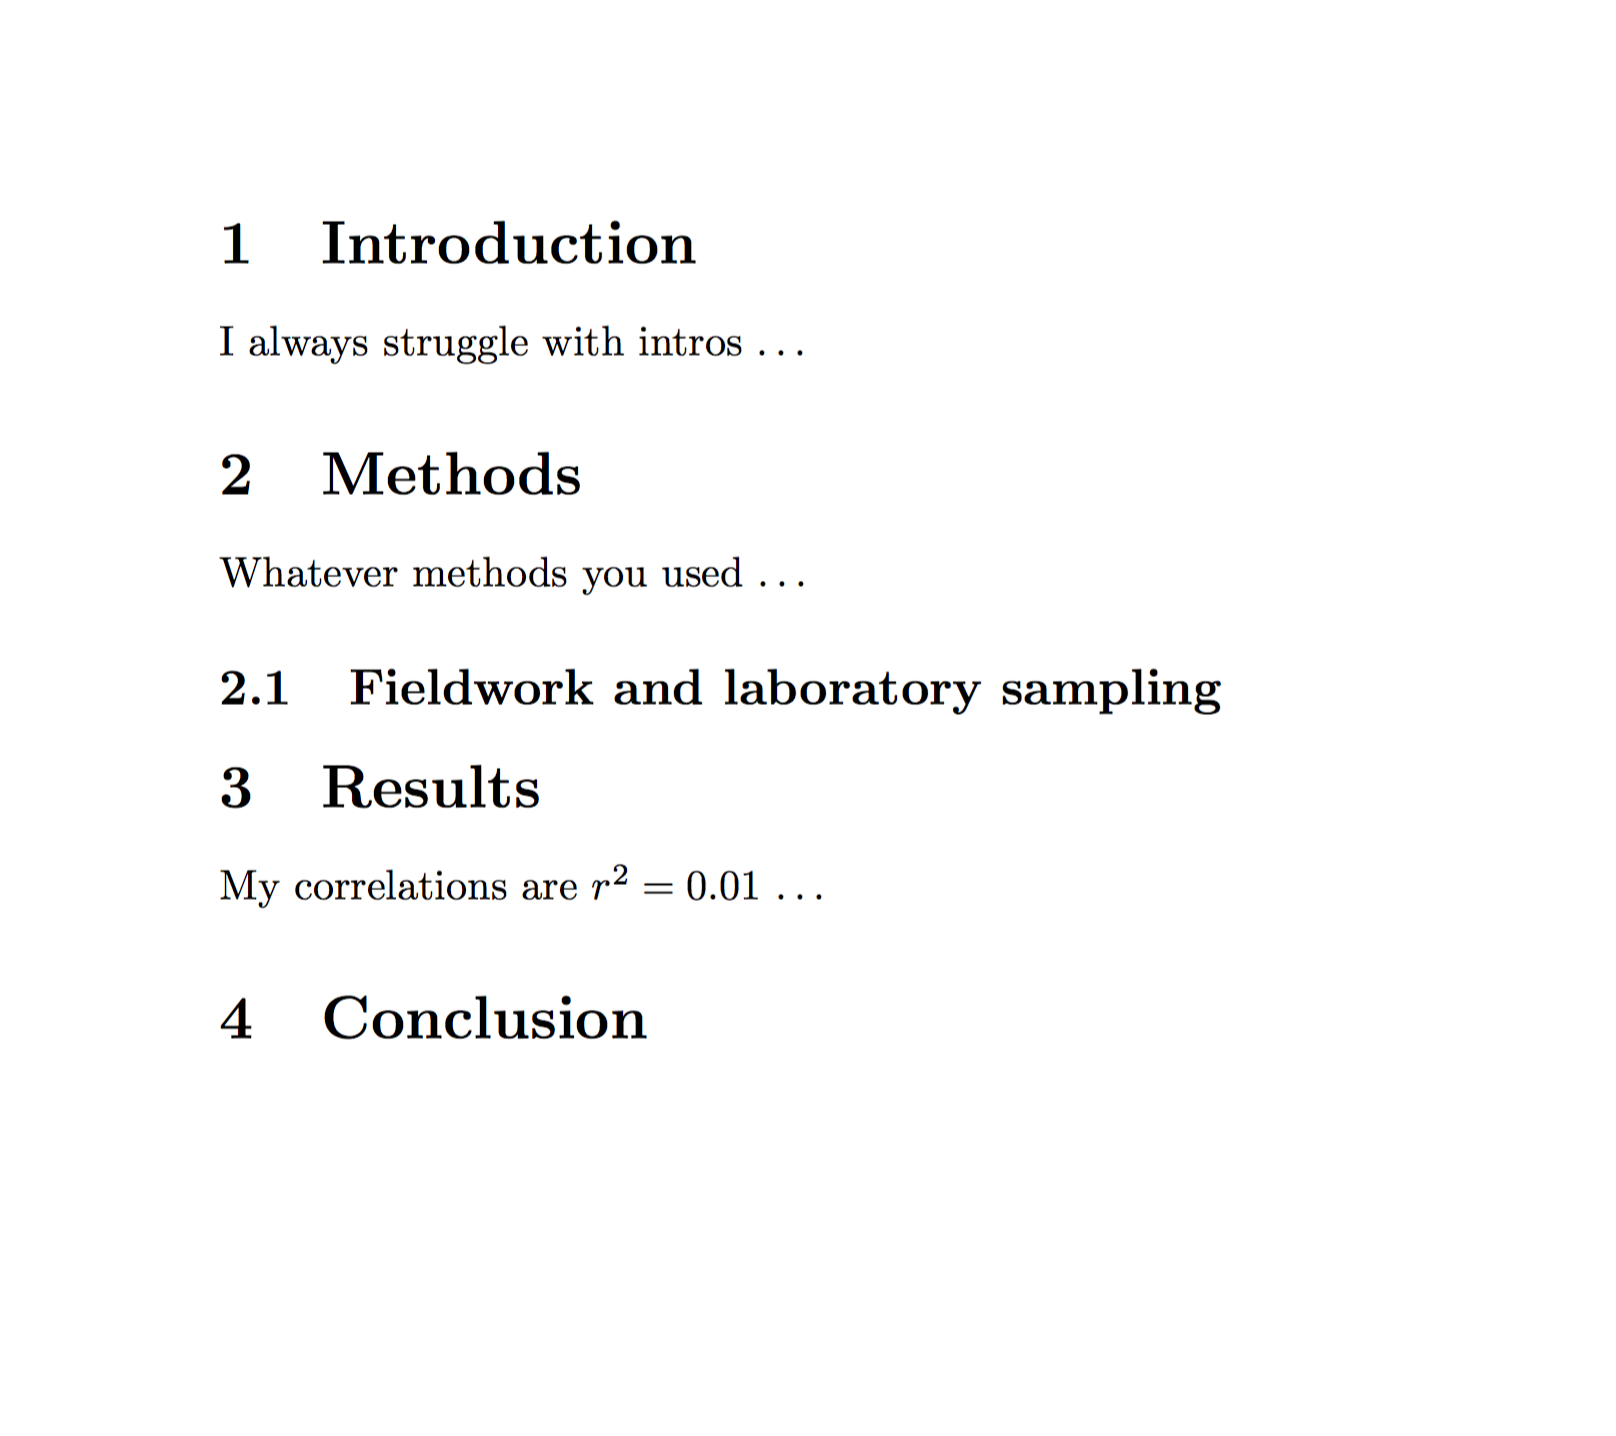
\includegraphics[width=100mm]{figures/example_2.png}
\end{figure}
\end{frame}


%------------------------------------------------
\begin{frame}[fragile]
\frametitle{Exercise 3: Overleaf}
\begin{itemize}
\item Open the exercise in Overleaf (Exercise3.tex).
\item Make the script look like Exercise3.pdf
\item  Hint: You can avoid enumerating equations by typing \verb|\begin{equation*}|.
\end{itemize}
\end{frame}

%------------------------------------------------
\begin{frame}[fragile]
\frametitle{To write papers or a thesis!}
Introducing the command: \color{blue}{\verb|\include{file}|}\color{black}{}. \\
\begin{itemize}
\item The \color{blue}{\verb|\include|}\color{black}{} command is used for selective inclusion of files. The \verb|file| argument is the first name of a file: file.tex.\\
\item Note that when you name the file inside the curly brackets, you do not need to add the extension. \\
\end{itemize}
\pause
Now, follow these instructions:
\begin{enumerate}
\item In Overleaf, find the folder \textbf{THESIS} and the file called \textbf{main.tex}, open it, and compile it. \\
\item Check the new packages and commands. \\
\item Learn how to collate different chapters of your thesis with one click (just sections here for the purporse of this exercise). \\
\end{enumerate}
\end{frame}


%------------------------------------------------
\begin{frame}[fragile]
\frametitle{Font sizes in \LaTeX}
\begin{figure}
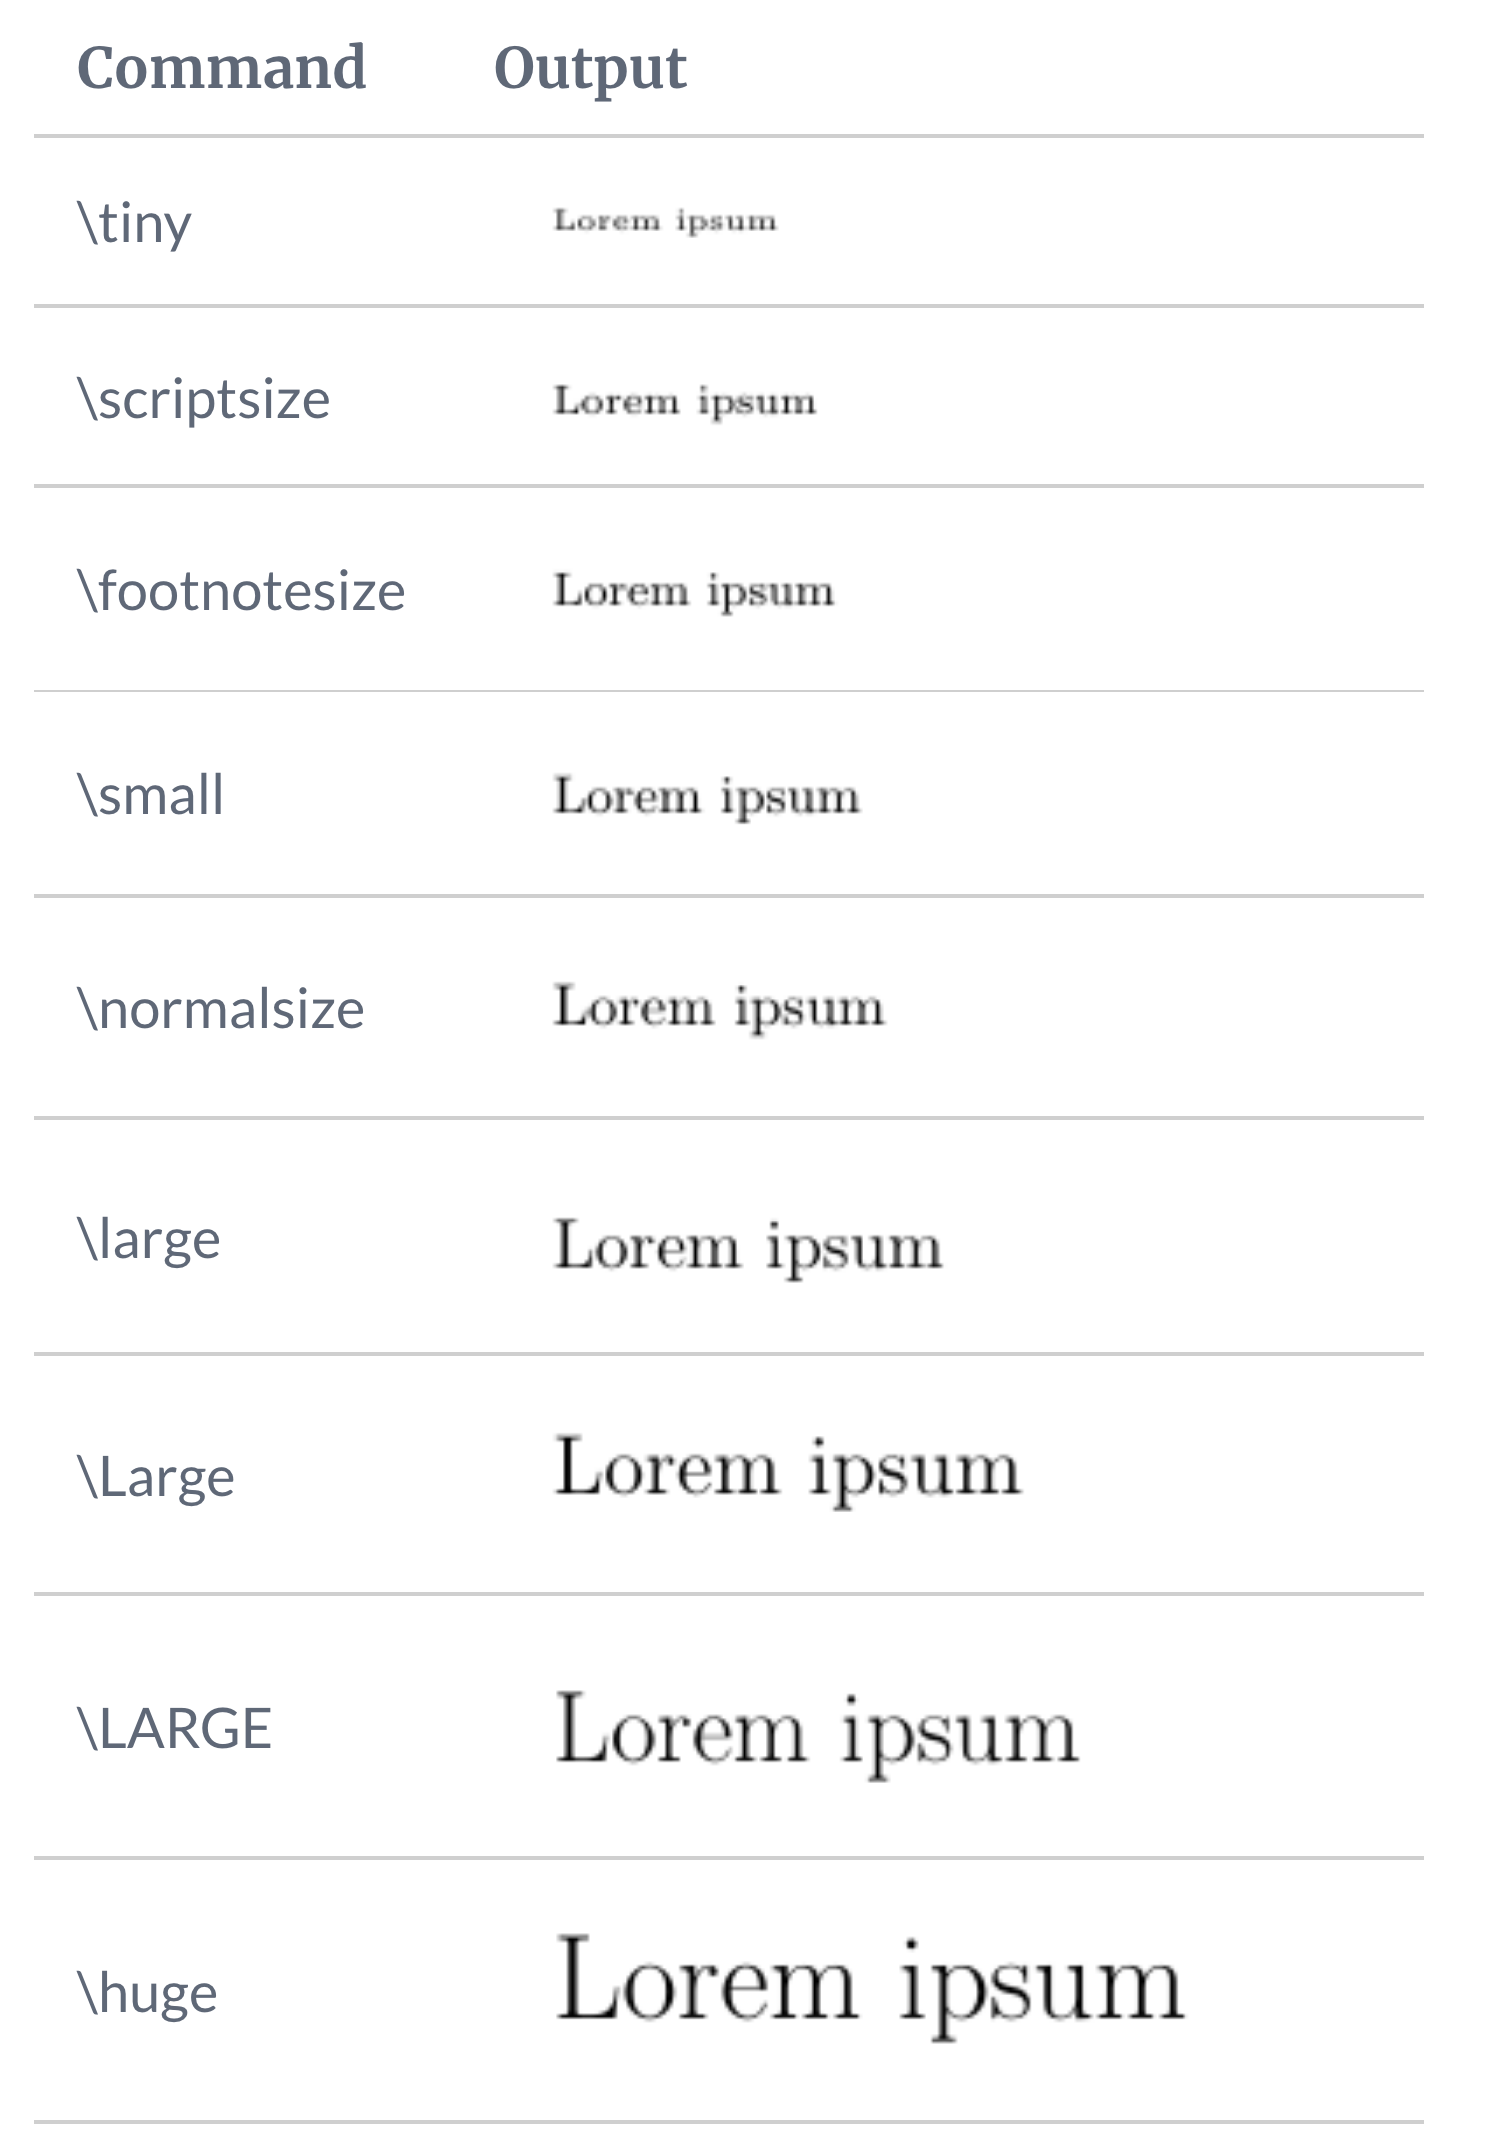
\includegraphics[width=56mm]{figures/Fonts.png}
\end{figure}
\end{frame}


%------------------------------------------------
\begin{frame}[fragile]
\frametitle{Last but not least: referencing}
%\LaTeX{} has three major bibliography management programs: \verb|biblatex|, \verb|natbib|, and \verb|bibtex|. The word BibTeX stands for a tool and a file format which are used to describe and process lists of references, mostly in conjunction with \LaTeX{}  documents. \\
%\vspace{1cm}
Firstly, you need to learn that in \LaTeX{} there are different types of documents. 
\begin{itemize}
\item The file .tex is the input file. \\
\item For referencing you will need another file with extension '.bib'. \\
\item A .bib file will contain the bibliographic information of your document. \\
\end{itemize}
\end{frame}

%------------------------------------------------
\begingroup
\footnotesize
\begin{frame}[fragile]
\frametitle{BibTeX: the .bib file}
\begin{itemize}
\item Your references in a .bib file in ‘bibtex’ database format would look like:
\end{itemize}
\begin{framed}
\begin{verbnobox}[\vbdelim]
@Article<{>Jacobson1999Towards,
author = <{>Van Jacobson<}>,
title = <{>Towards the Analysis of Massive Multiplayer Online
Role-Playing Games<}>,
journal = <{>Journal of Ubiquitous Information<}>,
Month = jun,
Year = 1999,
Volume = 6,
Pages = <{>75--83<}}>
\end{verbnobox}

\begin{verbnobox}[\vbdelim]
@InProceedings<{>Golledge2021Methodology,
author = <{>Nicholas Golledge and Liz Keller and
Stefan Jendersie<}>,
title = <{>A Methodology for the Study of
climate models<}>,
booktitle = <{>Proceedings of Climate<}>,
Month = jun,
Year = 2021<}>
\end{verbnobox}
\end{framed}
\end{frame}


%------------------------------------------------
\begin{frame}[fragile]
\frametitle{BibTeX: the \textit{key}}
Each entry in the .bib file has a \textit{key} that you can use to reference it in the document. For example,
\color{red}{Jacobson1999Towards} \color{black}{} is the \textit{key} for this article:
\begin{framed}
\begin{verbnobox}[\vbdelim]
@Article<{>Jacobson1999Towards,
author = <{>Van Jacobson<}>,
...
\end{verbnobox}
\end{framed}

\begin{itemize}
\item You would usually write a \textit{key} using the name, year, and title of the reference. \\
\end{itemize}
\end{frame}

%------------------------------------------------
\begin{frame}[fragile]
\frametitle{BibTeX: how to reference}

\begin{enumerate}
\item Define \color{blue}{\verb|\usepackage{natbib}|} \color{black}{} in the \textit{preamble}. This will allow you to use the commands \color{blue}{\verb|\citet|} \color{black}{and} 
\color{blue}{\verb|\citep|} \color{black}{}. \textit{Can you guess what is the difference between each command?}\\
\item You will need to use the command \color{blue}{\verb|\bibliography|} \color{black}{} and specify a  \color{blue}{\verb|\bibliographystyle|} \color{black}{}. \\
\end{enumerate}

\begin{framed}
\begin{verbnobox}[\vbdelim]
<\documentclass{>article<}>
<\usepackage{>natbib<}>
<\begin{>document<}>
<\citet{>Jacobson1999Towards<}>
show that <\ldots>. Clearly,
the study of climate requires modelling
<\citep{>Golledge2010Methodology<}>.
<\bibliography{>bib-example<}>
% if `bib-example' is the name of
% your bib file (note: do not put the extension .bib here)
<\bibliographystyle{>plainnat<}>
% try changing to abbrvnat
<\end{>document<}>
\end{verbnobox}
\end{framed}
\end{frame} 

%------------------------------------------------
\begin{frame}[fragile]
\frametitle{BibTeX: how to reference}
\begin{figure}
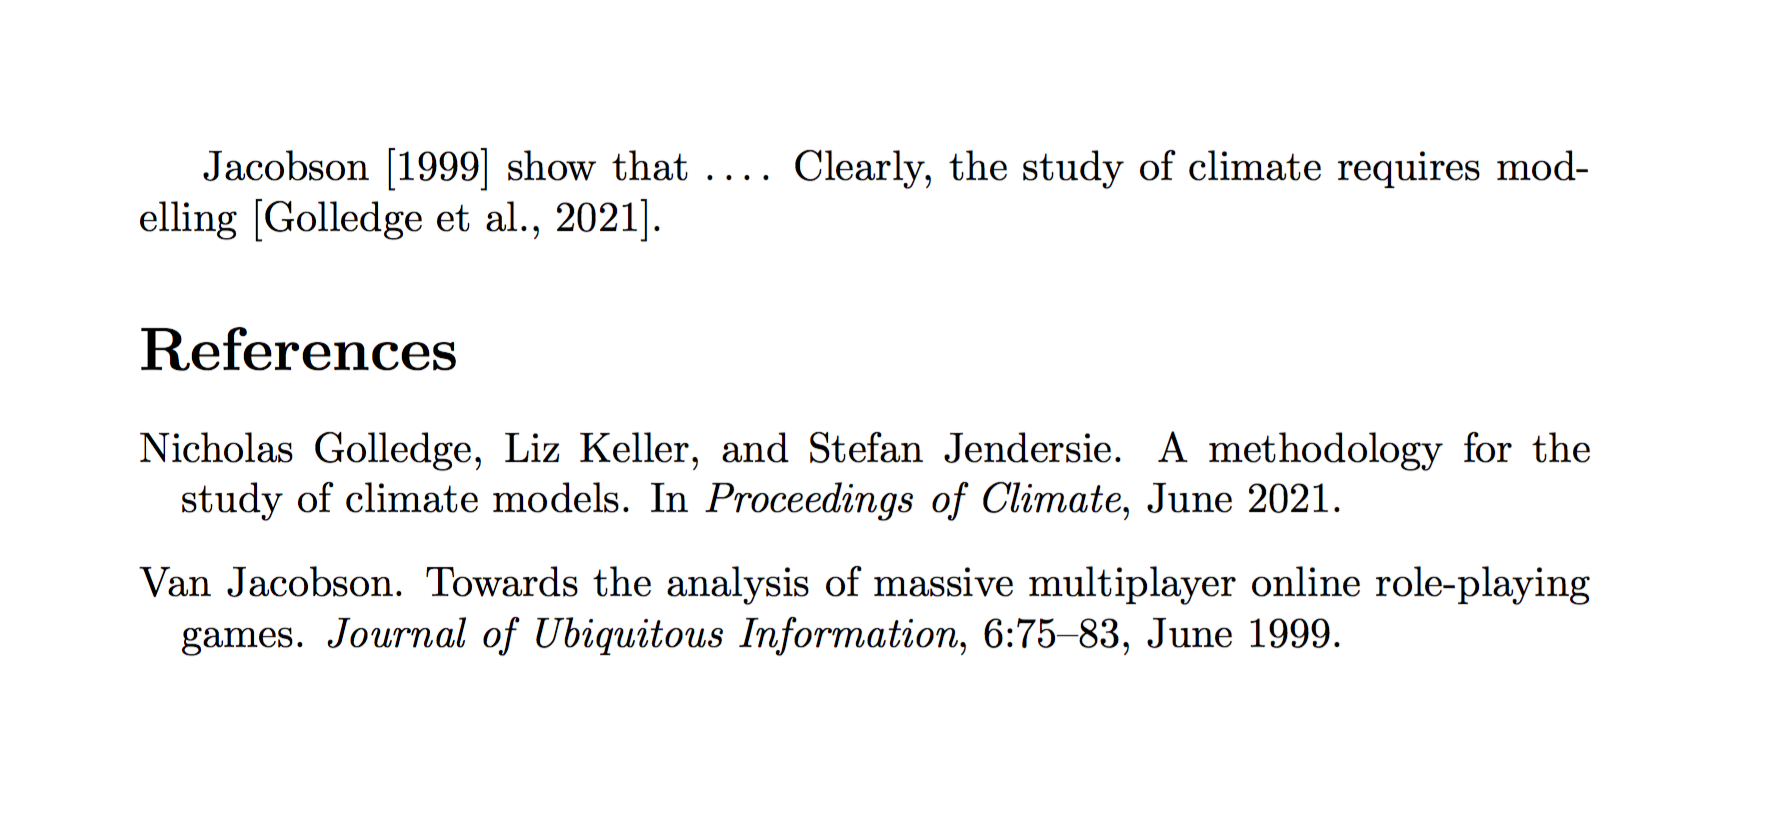
\includegraphics[width=120mm]{figures/Citing.png}
\end{figure}
You guessed right (maybe?): \color{blue}{\verb|\citet|} \color{black}{} cites as Author (year), while \color{blue}{\verb|\citep|} \color{black}{} cites as (Author, year).
\end{frame}



%------------------------------------------------
\begin{frame}[fragile]
\frametitle{Bibliography style}
There are many styles you can choose for your bibliography:
\begin{figure}
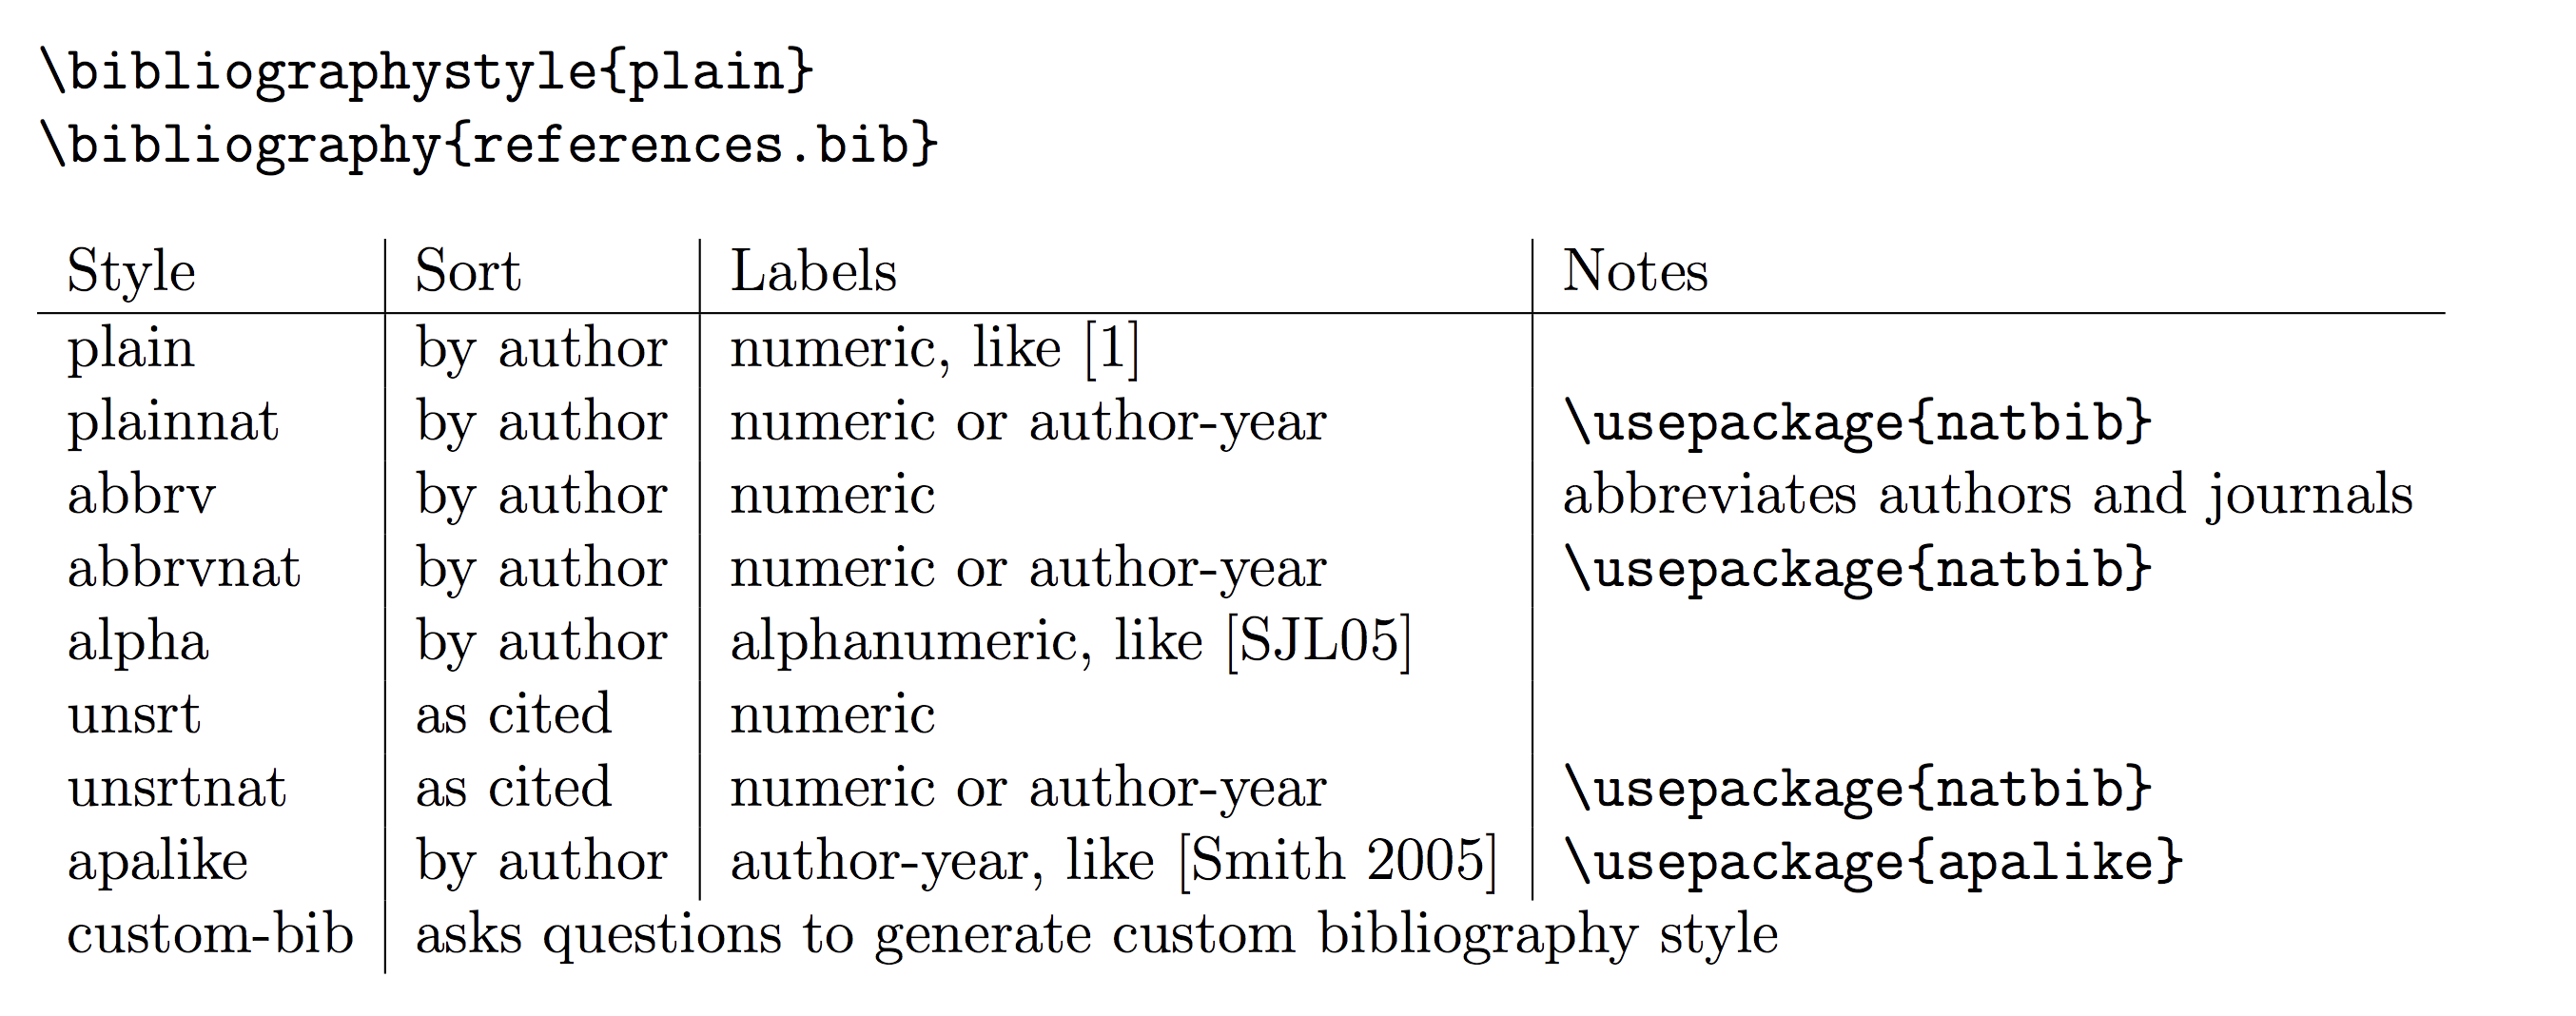
\includegraphics[width=100mm]{figures/bibliostyle.png}
\end{figure}
However, most journals or schools have their own style and it will come in a file '.bst'. 
\end{frame}

%------------------------------------------------
\begin{frame}[fragile]
\frametitle{How do journals work?}
Note that most journal's \LaTeX{} template will also come with a '.sty' file, which is the own style of the journal to define the layout of the paper. For example:
\begin{verbnobox}[\vbdelim]
<\documentclass{>copernicus<}> %there will be a file called copernicus.sty
<\usepackage{>natbib<}>
<\begin{>document<}>
%Your paper goes here
<\bibliographystyle{>copernicus<}> % a file called copernicus.bst
<\bibliography{>paper<}> %a file called paper.bib that you will create
<\end{>document<}>
\end{verbnobox}
\end{frame}


%------------------------------------------------
\begin{frame}[fragile]
\frametitle{Create your .bib file}
\begin{itemize}
\item Step 1: download your citation
\end{itemize}
\begin{figure}
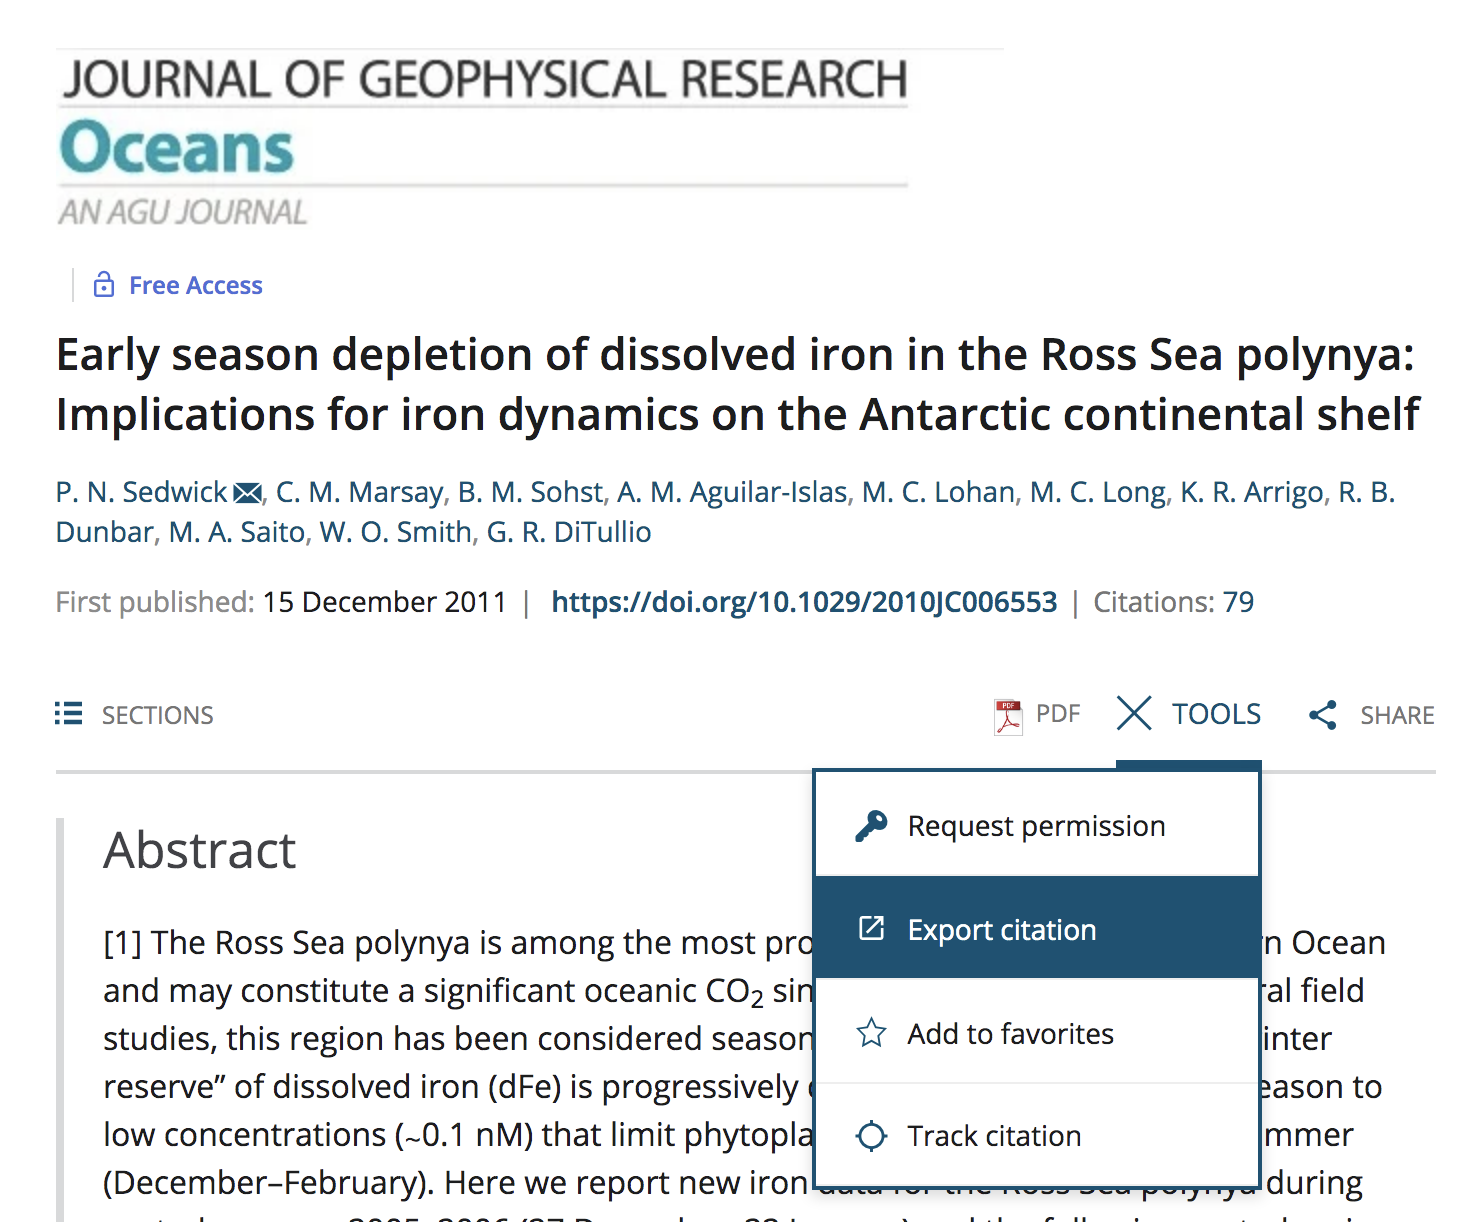
\includegraphics[width=80mm]{figures/Bib1.png}
\end{figure}
\end{frame}

%------------------------------------------------
\begin{frame}[fragile]
\frametitle{Create your .bib file}
\begin{itemize}
\item Step 2: choose the bibtex style
\end{itemize}
\begin{figure}
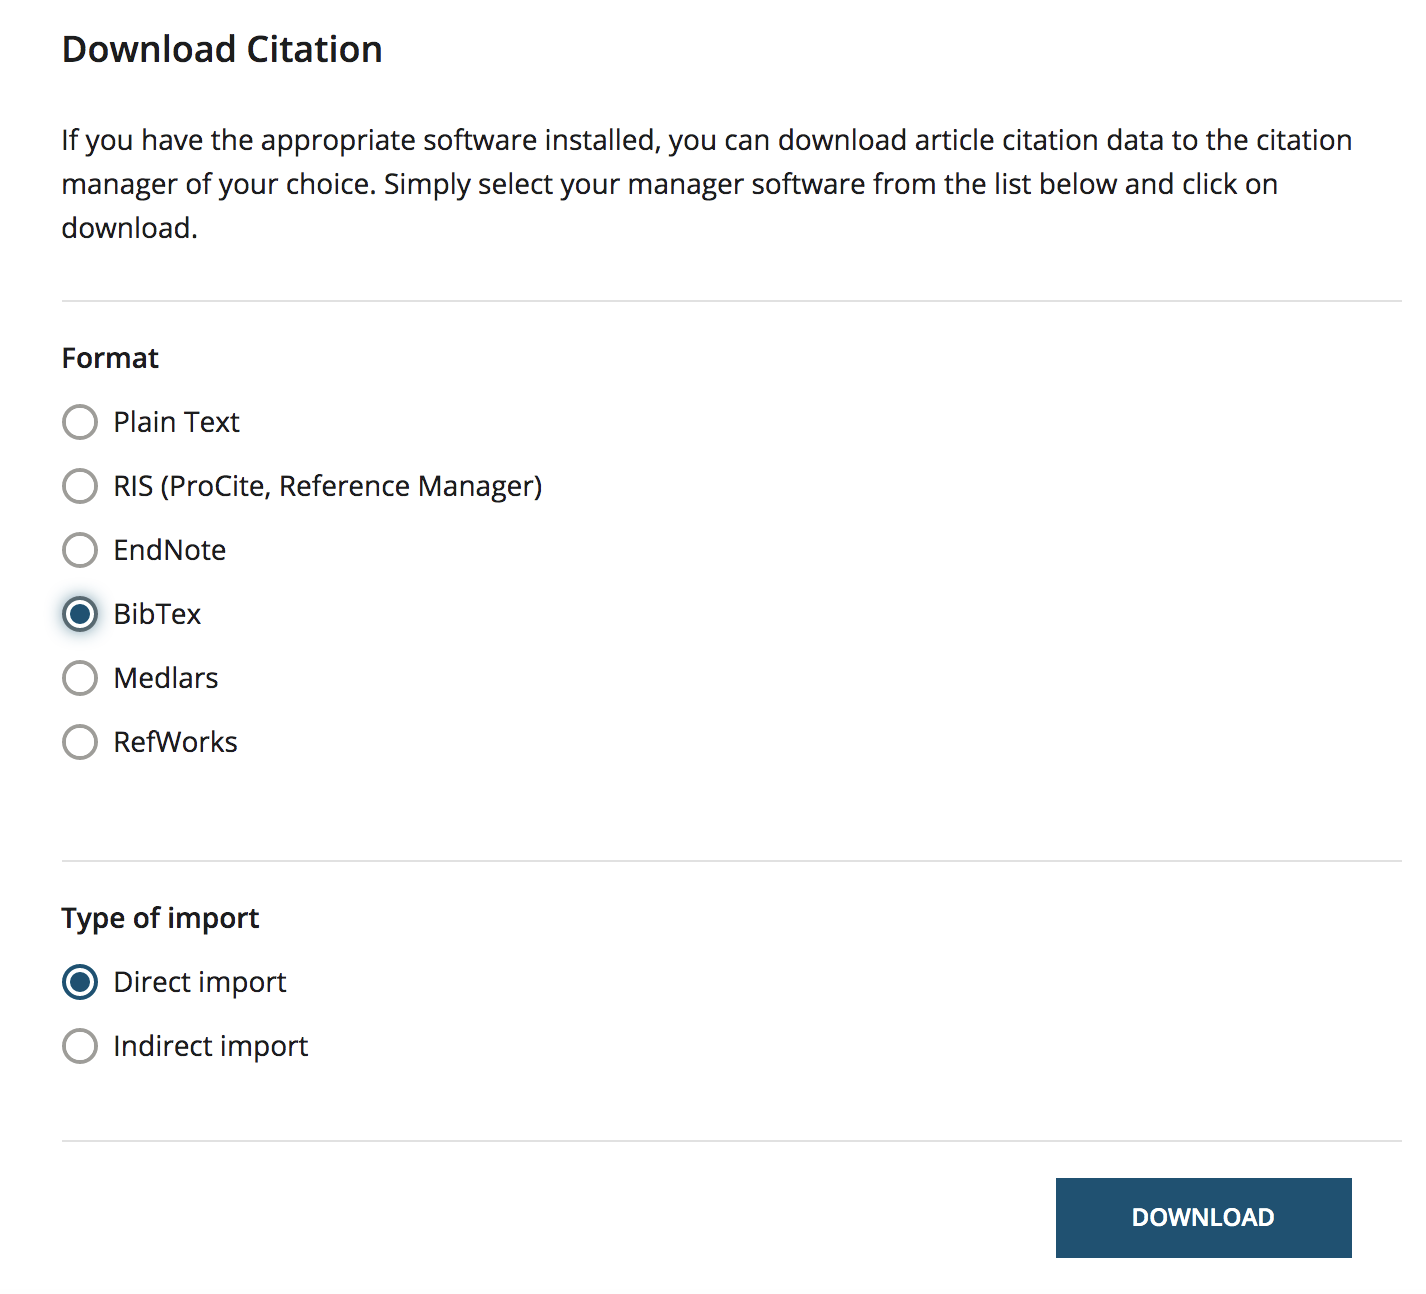
\includegraphics[width=80mm]{figures/Bib2.png}
\end{figure}
\end{frame}

%------------------------------------------------
\begin{frame}[fragile]
\frametitle{Create your .bib file}
\begin{itemize}
\item Step 3: personal choice, but I use BibDesk, an application that comes with TexShop (\LaTeX{} for Mac users).
\end{itemize}
\begin{figure}
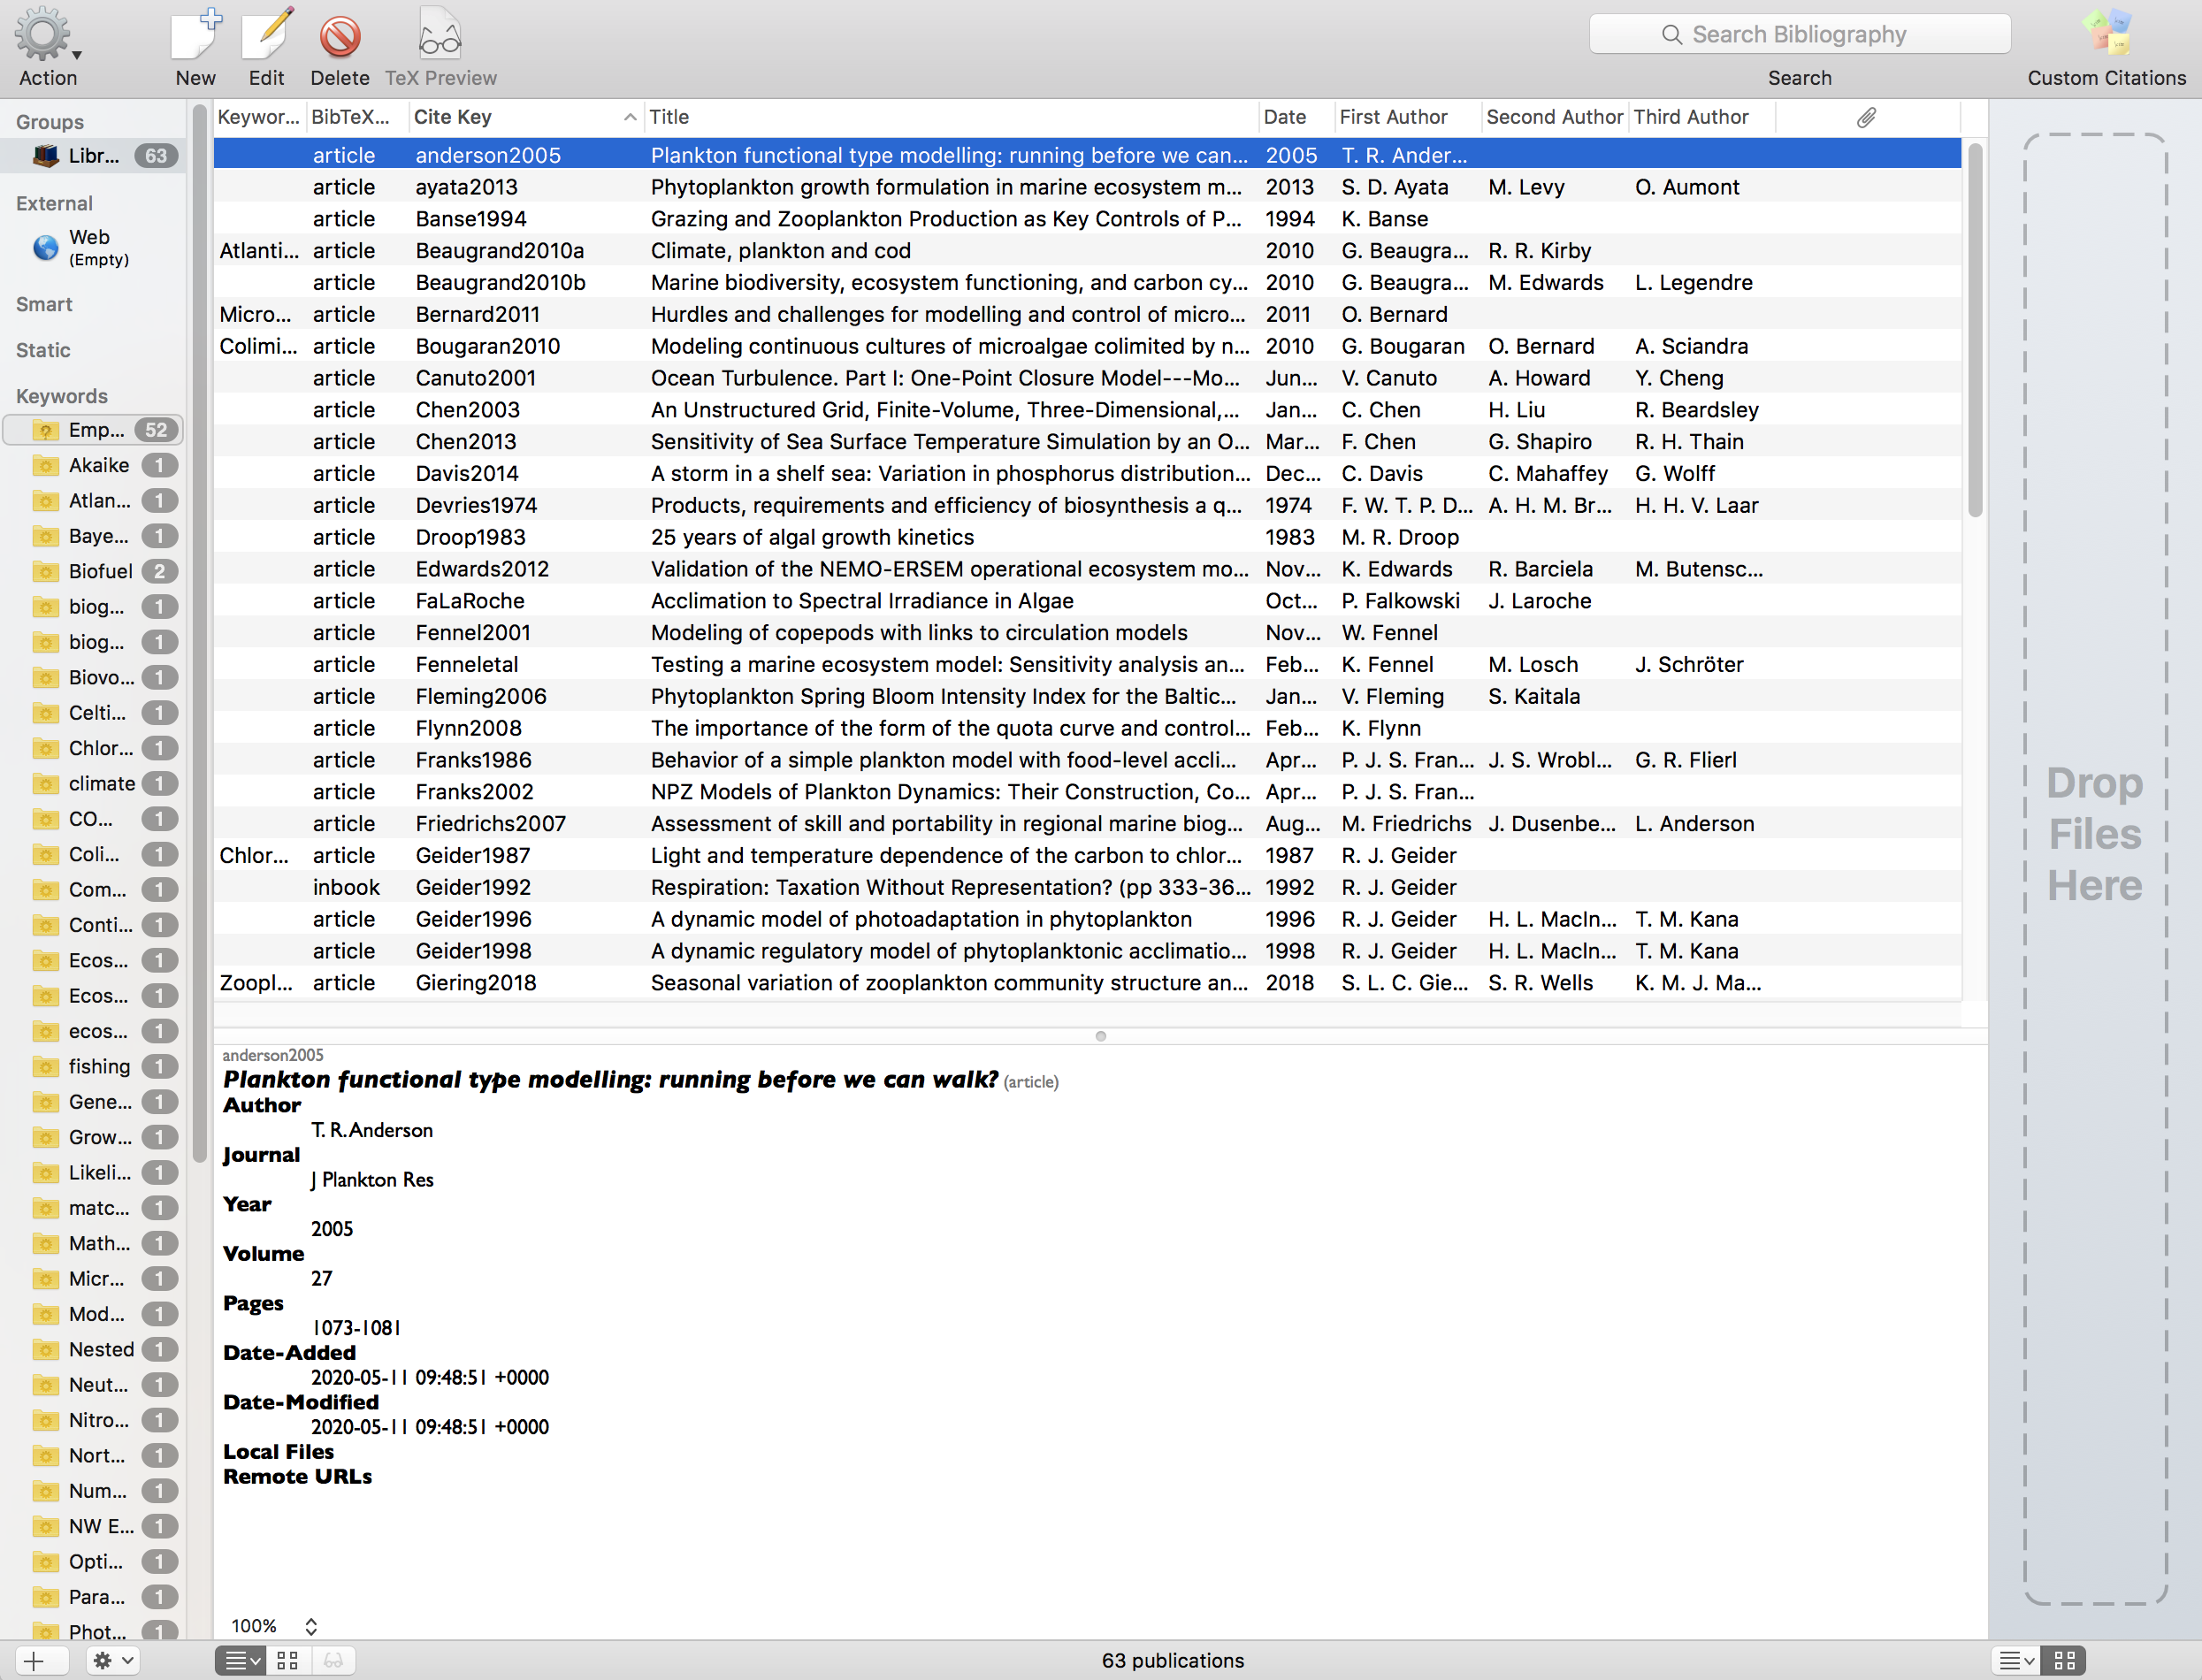
\includegraphics[width=90mm]{figures/BibDesk.png}
\end{figure}
\end{frame}

%------------------------------------------------

\begin{frame}[fragile]
\frametitle{Create your .bib file with BibDesk}
\begin{enumerate}
\item Open the exported Bibtex citation and go to the tab 'Publication' $\rightarrow$ 'New publication from file'.\\
\item Edit the cite-key to one of your choice. \\
\end{enumerate}
\begin{figure}
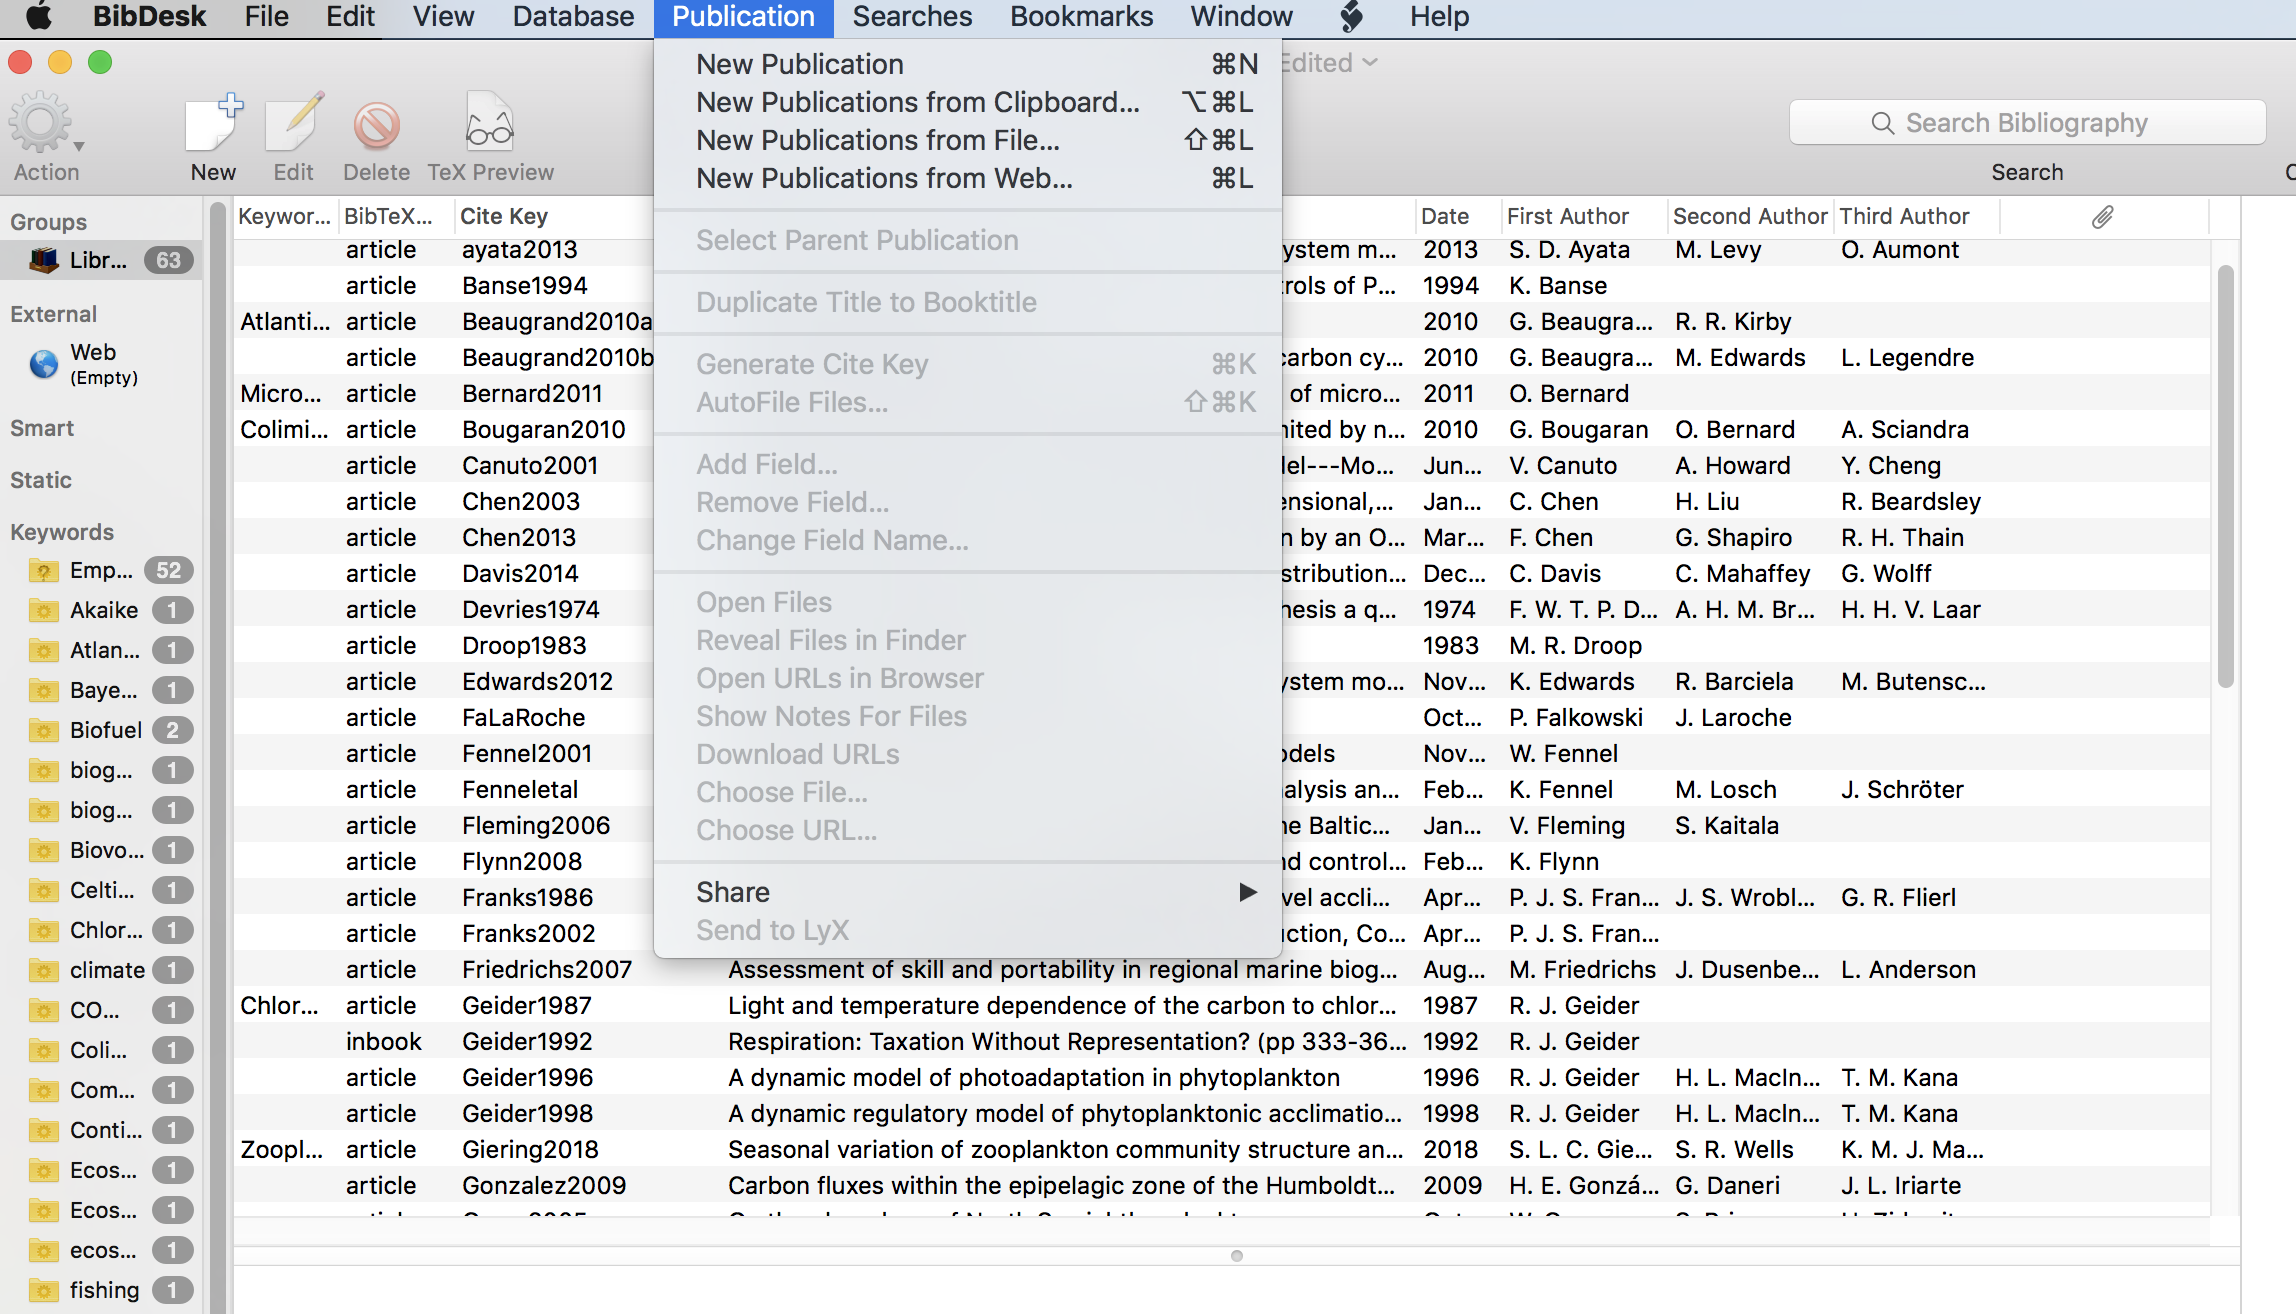
\includegraphics[width=100mm]{figures/BibDesk1.png}
\end{figure}
\end{frame}

%------------------------------------------------

\begin{frame}[fragile]
\frametitle{Create your .bib file with BibDesk}
\begin{enumerate}
  \setcounter{enumi}{2}
\item Save document as '.bib' and call it in your main.tex with \color{blue}{\verb|\bibliography|} \color{black}{} and \color{blue}{\verb|\bibliographystyle|} \color{black}{}. Which you already learned how to do! \\
\item To compile: latex, bibtex, latex, latex. Yes, latex twice!
\item Your references from .bib will only appear when you call them in the text (using \color{blue}{\verb|\citep|} \color{black}{}, \color{blue}{\verb|\citet|} \color{black}{}). \\
\end{enumerate}
\begin{figure}
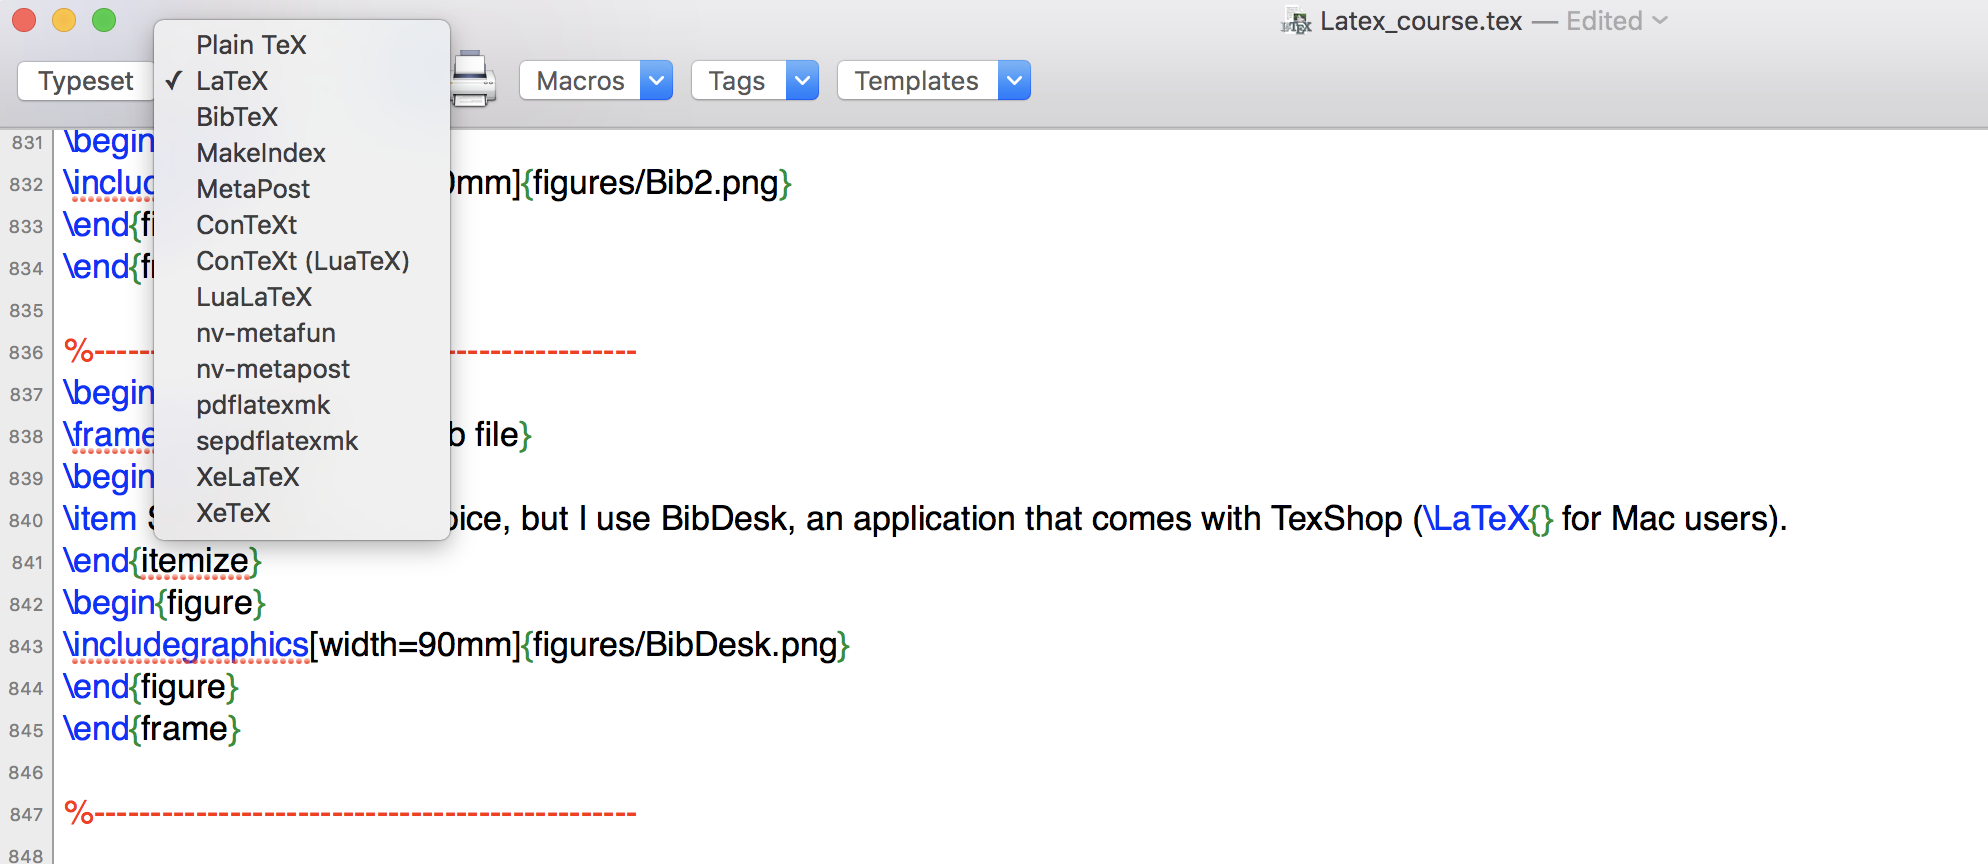
\includegraphics[width=90mm]{figures/compile.png}
\end{figure}
\vspace{0.5cm}
\textit{Homework: how to import your references in Unix or Windows?}
\end{frame}

%------------------------------------------------
\begin{frame}
\begin{figure}
\includegraphics[width=100mm]{figures/Frodo.jpeg}
\end{figure}
\end{frame}



%----------------------------------------------------------------------------------------

